% =============================================================================
%  Supplementary Section S7: late infusions.
%  Order: protocol; without illness (with the slack figure); by setting (Table stab:delays and
%  the corner table); during an illness; sensitivity to k; what the results do and do not say.
%  Sources: audit/brief_2026-10-01/out/t55_infusion_tolerance.txt (and t55 script header),
%  out/t54_dose_timing.txt (quasi-static slack, skipped dose); pi_note/pi_note.tex Result 5 and
%  tab:delay; pi_note/figure_guide.tex Figure 5; REPORT.md R-T.
% =============================================================================
\section{Late infusions}
\label{si:s7}

This section gives the simulation protocol and the full results behind the main text's analysis of
late and skipped infusions. Supplementary Section~\ref{si:s6} judged an interval by a quasi-static
condition on the trough. Here we integrate the two-state carnitine model through time
(Eq.~\eqref{seq:s1-twostate}), so that the metabolite is followed through a long gap between
infusions and through an illness.

% -----------------------------------------------------------------------------
\subsection{Simulation protocol}
\label{si:s7:protocol}

\paragraph{Model and dose train.} The two-state system of Eq.~\eqref{seq:s1-twostate}, with
metabolite $m$ and available carnitine $c$, was integrated at the baseline load of 600\um, with the
delivered increment $\Delta(t)$ of Eq.~\eqref{seq:s1-delta} added to the patient's own capacity in
the enzyme term. Eight infusions every 14 days settle the dose cycle. The next infusion is then given
$d$ days late, or skipped (the following infusion arriving 28 days after the last on-time one), and
infusions resume every 14 days counted from the late one.

\paragraph{Usual and gap peaks.} The usual peak is the highest metabolite level in the regular
14-day cycle before the last on-time infusion, reached just before that infusion; for a patient with
no enzyme of their own at the assumed dose, nominal constants, $k=1$\,d$^{-1}$ and a 4.3-day
half-life it is 40.4\uM. The gap peak is the highest
level from the last on-time infusion until 3 days after the late one. During an illness the window
runs on to the infusion after the late one, because the end of the illness can bring a later peak,
when the raised load meets the next trough of the delivered enzyme. Results are reported as the gap
peak divided by the usual peak of the same setting, so that each setting is judged against its own
yardstick; at $k=1$\,d$^{-1}$ the usual peaks of a patient with no enzyme of their own range from 21
to 342\uM\ across the corners of the carnitine constants, doses and half-lives.
% src: audit/brief_2026-10-01/t55_infusion_tolerance.py:11-19 (8 doses; late or skipped; window to 3 d after the late dose, extended during illness to the next dose), :133 (usual = max over [pre[-2], pre[-1]), the cycle before the last on-time dose); pi_note/pi_note.tex:452-454 (usual peak reached just before each on-time infusion); manuscript/main.tex:770 (cycle before the last on-time infusion); out/t55_infusion_tolerance.txt:65 (usual 40.4 uM), :111-153 (usual peaks 21.4-342.0 uM, k = 1); REPORT.md:1169 (usual peak reached just before each on-time dose), :1188 (usual peaks 21-342 uM across the corners)

\paragraph{Illness.} For illustration, an intercurrent illness raises the load to 1.5 times
baseline (900\um) for 14 days, starting on the day the infusion is due.

\paragraph{Criteria.} Three criteria give the number of days an infusion can be late.
\begin{enumerate}[nosep,leftmargin=1.6em]
\item \emph{Trough condition.} The capacity at the end of the gap, $\theta$ plus the delivered
enzyme left, must stay above $\thci$ (Eq.~\eqref{seq:s6-condition}). A dose $d$ days late lets the
fortnightly trough decay to $\dtr(14)\,e^{-\lambda d}$, so the slack is
\begin{equation}
\label{seq:s7-dq}
d_{\mathrm{tr}}(\theta)\;=\;\frac{1}{\lambda}\,\ln\frac{\dtr(14)}{\thci-\theta},\qquad 0\le\theta<\thci ,
\end{equation}
which is negative (the condition fails with the infusion on time) when $\dtr(14)<\thci-\theta$,
and infinite when $\theta\ge\thci$.
\item \emph{Peak doubling.} The gap peak must stay below twice the usual peak, a yardstick chosen
because the model does not define a harmful metabolite level. The delay at which the peak doubles
was found by bisection to within 0.025\,d.
\item \emph{Separatrix.} The gap peak must stay below the unstable steady state of the carnitine
model at the patient's usual trough capacity, $\theta+\dtr(14)$, beyond which the metabolite would
keep rising on its own, or below the validity limit if that is lower.
\end{enumerate}
The model is used below $m\approx5.5\,M_i$ (Section~\ref{si:s1-carn}): 1650\uM\ at the nominal
$M_i=300$\uM\ and 825\uM\ at $M_i=150$\uM. Peaks beyond this limit are flagged and not quoted as
multiples.
% src: audit/brief_2026-10-01/t55_infusion_tolerance.py:21-35 (three criteria; d_q = ln(Delta_tr(14)/(theta_crit - theta))/lambda; bisection; separatrix at the usual trough capacity or the validity limit, whichever lower), :156-171 (bisection tol 0.05, midpoint within 0.025 d), :14-19 (5.5 M_i: 1650 / 825 uM; illness 1.5 x baseline for 14 d from the due day); out/t55_infusion_tolerance.txt:4,60; manuscript/main.tex:773 (bisection to within 0.025 d)

\paragraph{Settings.} Doses: the assumed $D=6000$\um\ and $D=2672$\um, the fortnightly dose capped at
the ceiling at a 3.5-day half-life (Supplementary Section~\ref{si:s6:ceiling}; at 4.3 days it slightly
exceeds the ceiling). Carnitine constants: nominal, and the eight corners of the assumed ranges with
$R_0$ re-derived at each. Half-lives: 3.5 days (the assumed design value of the identifiability and
sampling analyses) and 4.3 days (the likely hepatic value). Residual capacities: 0, 1, 2.5 and 5\% of normal
(0, 30, 75 and 150\um). Conjugation rate: $k=1$\,d$^{-1}$, the model default, and $k=10$\,d$^{-1}$,
close to the limit in which carnitine follows the metabolite instantly (Supplementary
Table~\ref{stab:s1-kcost}). Because 5\% of normal (150\um) lies only 0.8\um\ below the nominal
$\thci$, the trough slack of that patient is very sensitive to $\theta$ (31.5 days at $\theta=150$\um,
21 days at 145\um\ at a 3.5-day half-life); the dynamic criteria are not.
% src: audit/brief_2026-10-01/t55_infusion_tolerance.py:6-8,35-40 (k = 1 default; 5 % row 0.8 uM/d below theta_crit; 31.5 d at 150, 21 d at 145, which eq. seq:s7-dq gives at 3.5 d; worst corner K_c 25, M_i 150, rho_0 1; D = 2672 admissible at 5 %); pi_note/pi_note.tex:515-516 (D = 2672 slightly exceeds the ceiling at 4.3 d: peak 2672/(1 - 2^(-14/4.3)) = 2984 > 2850); out/t55_infusion_tolerance.txt:8-9

% -----------------------------------------------------------------------------
\subsection{Without illness}
\label{si:s7:noill}

At the assumed dose, nominal constants, $k=1$\,d$^{-1}$ and a 4.3-day half-life, each day of delay
multiplies the peak by a nearly constant factor of about 1.1, so the absolute rise grows with the
length of the gap.
For a patient with no enzyme of their own the peak is 1.1, 1.2 and 1.4 times its usual value one, two
and three days late, 1.9 and 2.1 times six and seven days late, and 5.1 times when the infusion is
skipped; at 2.5\% of normal the same delays give 1.1, 1.2, 1.3, 1.8, 1.9 and 3.4 times. The peak
doubles after 6.5, 6.9, 7.5 and 8.8 days at 0, 1, 2.5 and 5\% of normal (5.3, 5.9, 6.8 and 8.8 days at
a 3.5-day half-life).
% src: audit/brief_2026-10-01/out/t55_infusion_tolerance.txt:179 (0 %: 1.0 1.1 1.2 1.4 1.5 1.7 1.9 2.1 ... 5.1), :182 (2.5 %: 1.0 1.1 1.2 1.3 1.5 1.6 1.8 1.9 ... 3.4), :13-20 (2x, k = 1: 5.3/5.9/6.8/8.8 at 3.5 d; 6.5/6.9/7.5/8.8 at 4.3 d); pi_note/figure_guide.tex:559-561,593-595 (1.1, 1.2, 1.4, 1.9, 2.1; near-constant factor about 1.1)

A skipped infusion raises the peak 5.1, 4.2, 3.4 and 2.7 times at 0, 1, 2.5 and 5\% of normal at
4.3 days, and 10.2, 6.6, 4.0 and 2.6 times at 3.5 days. Once infusions resume, the metabolite returns
to its usual cycle in every setting computed. For a patient with no enzyme of their own at 4.3 days,
after a skipped infusion the first resumed cycle peaks 1.068 times the usual level and the next
1.007 times; after a seven-day delay, 1.050 and 1.005 times; after a three-day delay, 1.028 and
1.003 times. In the model a late or skipped infusion therefore leaves no lasting effect, although
this does not show that the gap itself was harmless.
% src: audit/brief_2026-10-01/out/t55_infusion_tolerance.txt:64-71 (skipped 10.2/5.1, 6.6/4.2, 4.0/3.4, 2.6/2.7), :62-104 ('back' column: last cycle peak equals the usual peak, to within 1 uM, in every row), :173-177 (booked dose, nominal, k = 1, 4.3 d, no own enzyme: 1.068/1.007; 1.050/1.005; 1.028/1.003); out/t54_dose_timing.txt:109-113 (the next dose restores the cycle, which does not show the gap was harmless)

At the assumed dose and nominal constants, for a patient with no enzyme of their own, the trough
condition fails after 9.5 days at 4.3 days, later than the peak doubles (6.5 days), and after 4.9
days at 3.5 days, before the peak doubles (5.3 days). A skipped infusion
leaves 73.4\um\ of delivered enzyme at the end of the 28-day gap at 4.3 days, so the trough condition
then holds only for patients above 77.3\um\ of their own (2.6\% of normal); at 3.5 days 25.0\um\ is
left and the condition needs more than 125.8\um\ (4.2\%). At $D=2672$ the corresponding values are
32.7\um\ and 118.1\um\ (3.9\%) at 4.3 days, and 11.1\um\ and 139.6\um\ (4.7\%) at 3.5 days.
Supplementary Fig.~\ref{sfig:s7-slack} shows how both slacks change with the half-life.
% src: audit/brief_2026-10-01/out/t55_infusion_tolerance.txt:13,17 (0 %: trough 4.9 d and 2x 5.3 d at 3.5 d; trough 9.5 d and 2x 6.5 d at 4.3 d); out/t54_dose_timing.txt:33-39 (skipped dose: 25.0 -> 125.8 (4.2 %); 73.4 -> 77.3 (2.6 %); 11.1 -> 139.6 (4.7 %); 32.7 -> 118.1 (3.9 %))

\begin{figure}[tbp]
\centering
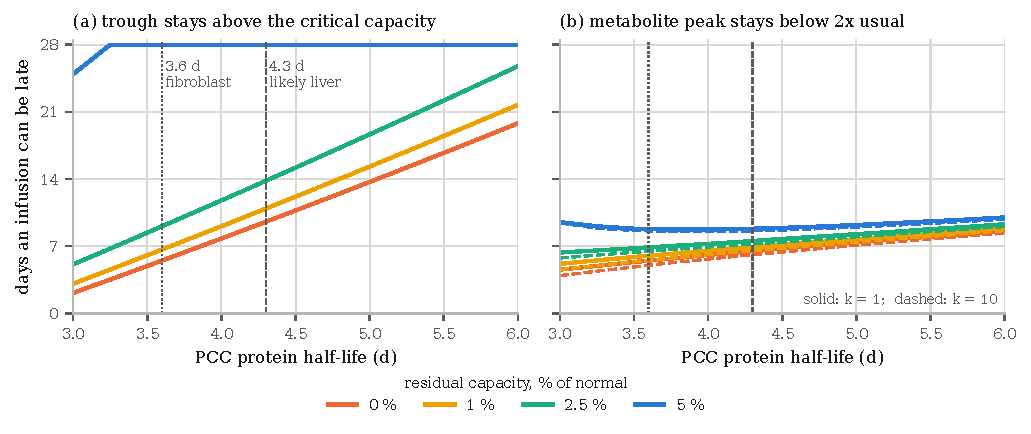
\includegraphics[width=\linewidth]{pi_tolerance_slack.pdf}
\caption{\label{sfig:s7-slack}Days an infusion can be late, against the half-life of the delivered
PCC protein, in the two-state carnitine model at the assumed dose ($D=6000$\um\ per fortnight),
nominal carnitine constants and baseline load, for patients with 0, 1, 2.5 and 5\% of normal capacity
of their own (colours). (a) Days until the trough condition fails, that is until the patient's own
capacity plus the delivered enzyme left at the end of the gap falls below the intrinsic critical
capacity $\thci=150.8$\um\ (Eq.~\eqref{seq:s7-dq}). The vertical axis is capped at 28 days (two
missed infusions); the patient at 5\% of normal reaches the cap from a half-life of about 3.25\,d,
because their own capacity lies only 0.8\um\ below $\thci$. (b) Days until the metabolite's highest
level in the gap reaches twice its usual on-therapy peak, without illness; solid lines $k=1$\,d$^{-1}$
(the model default), dashed lines $k=10$\,d$^{-1}$. Vertical lines: the human fibroblast half-life,
3.6\,d (dotted), and the likely hepatic value, 4.3\,d (dashed). A skipped infusion is 14 days late.
The trough slack rises steeply with the half-life (at 4.3\,d, about 9 to 14 days for 0 to 2.5\% of
normal), whereas the doubling delay changes more slowly, staying between about 4 and 10 days over
half-lives of 3 to 6\,d.}
\end{figure}
% src: audit/brief_2026-10-01/out/t55_infusion_tolerance.txt:155-171 (figure data, booked dose, nominal constants; capped at 28 d; q 5 %: 24.9 d at 3.00 d, 28.2 d at 3.25 d; 2x between 3.9 and 10.0 d over 3-6 d, k = 1 and k = 10; q at 4.25-4.50 d: 9.2-10.7, 10.6-12.2, 13.5-15.2), :17-19 (4.3 d trough 9.5/10.9/13.8 d); audit/brief_2026-10-01/pi_note/fig/pi_tolerance_slack.png (panel titles, legends, vertical lines; no model names in the figure)

% -----------------------------------------------------------------------------
\subsection{By setting}
\label{si:s7:settings}

Supplementary Table~\ref{stab:delays} gives the three slacks for every dose, half-life and capacity,
at the nominal constants and at the corner with the highest critical capacity ($K_c=25$\uM,
$M_i=150$\uM, $\rho_0=1$; $\thci=232.1$\um). Having the highest threshold, that corner is the least
favourable for the trough condition in every setting. For the doubling, computed at all eight
corners only for a patient with no enzyme of their own at $k=1$\,d$^{-1}$, it is also the least
favourable at $D=2672$, but at the assumed dose other corners bring the doubling sooner.
Supplementary Table~\ref{stab:s7-corners} therefore gives both slacks at all eight corners for
that patient.
% src: audit/brief_2026-10-01/out/t55_infusion_tolerance.txt:106-153 (per-corner values, no own enzyme, k = 1; (25, 150, 1) sets the trough columns and the D = 2672 doubling); t55_infusion_tolerance.py:231-244; REPORT.md:1188

Taking, for a patient with no enzyme of their own, the shortest slack over the corners for each
criterion separately, the trough condition fails before the peak doubles in six of the eight
combinations of dose, constants and half-life, all but the assumed dose at 4.3 days (9.5 against 6.5
days at the nominal constants, 6.9 against 4.5 days at the least favourable). In the least favourable
setting, $D=2672$ with the least favourable constants and a 3.5-day half-life, the peak of a patient
with no enzyme of their own doubles after 2.4 days, and the trough condition already fails with the
infusion on time for patients with 0 or 1\% of normal; at a 4.3-day half-life the peak of that
patient doubles after 4.3 days and the trough condition fails after 1.8 days. In every setting of
Supplementary Table~\ref{stab:delays}, at both values of $k$, the peak doubles before the metabolite
reaches the validity limit or the separatrix at the usual trough capacity (compare its doubling and
separatrix columns). Once the capacity at the end of the gap has fallen below
$\thci$, however, there is no separatrix, and the metabolite rises on its own until the infusion
arrives.
% src: audit/brief_2026-10-01/out/t55_infusion_tolerance.txt:120,131,142,153 (minima: 2x 4.5/trough 6.9; 4.0/2.7; 4.3/1.8; 2.4/fails on time), :11-53 (all settings; 2x < sep throughout, k = 1 and k = 10), :46-47 (fails on time at 0 and 1 %), :50 (4.3 d, 0 %: trough 1.8, 2x 4.3); pi_note/pi_note.tex:495-503,523-536 (no tipping point once below the critical capacity); REPORT.md:1179-1188

\begingroup
\footnotesize
\setlength{\tabcolsep}{5pt}
\begin{longtable}{@{}llccccc@{}}
\caption{\label{stab:delays}Days an infusion can be late, by setting, in the two-state carnitine
model at baseline load (600\um), without illness. Trough: until the capacity at the end of the gap
falls below $\thci$ (Eq.~\eqref{seq:s7-dq}); ``on time'' means the condition already fails with the
infusion on time. Doubling: until the gap peak reaches twice the usual peak of that setting, at
$k=1$ and $k=10$\,d$^{-1}$. Separatrix: until the gap peak passes the unstable steady state at the
patient's usual trough capacity, or the validity limit if lower (1650\uM\ nominal, 825\uM\ at the
corner); $>28$: not within 28 days. Capacities are per cent of normal (3000\um). Least favourable:
the corner $K_c=25$\uM, $M_i=150$\uM, $\rho_0=1$ ($\thci=232.1$\um, against 150.8 nominal), with $R_0$
re-derived; at the assumed dose other corners bring the doubling sooner for a patient with no enzyme
of their own (Supplementary Table~\ref{stab:s7-corners}). $D=2672$\um\ is the fortnightly dose capped at
the ceiling at a 3.5-day half-life.}\\
\toprule
& & & \multicolumn{2}{c}{doubling} & \multicolumn{2}{c}{separatrix} \\
\cmidrule(lr){4-5}\cmidrule(l){6-7}
$t_{1/2}$ & capacity & trough & $k=1$ & $k=10$ & $k=1$ & $k=10$ \\
\midrule
\endfirsthead
\multicolumn{7}{@{}l}{\emph{Supplementary Table~\ref{stab:delays}, continued}}\\
\toprule
& & & \multicolumn{2}{c}{doubling} & \multicolumn{2}{c}{separatrix} \\
\cmidrule(lr){4-5}\cmidrule(l){6-7}
$t_{1/2}$ & capacity & trough & $k=1$ & $k=10$ & $k=1$ & $k=10$ \\
\midrule
\endhead
\bottomrule
\endfoot
\multicolumn{7}{@{}l}{\emph{Assumed dose, $D=6000$\um; nominal constants}}\\
3.5\,d & 0\% & 4.9 & 5.3 & 4.8 & 18.4 & 16.4 \\
 & 1\% & 6.0 & 5.9 & 5.4 & 21.1 & 18.7 \\
 & 2.5\% & 8.4 & 6.8 & 6.4 & 27.2 & 24.1 \\
 & 5\% & 31.5 & 8.8 & 8.6 & $>28$ & $>28$ \\
4.3\,d & 0\% & 9.5 & 6.5 & 6.1 & 23.7 & 21.6 \\
 & 1\% & 10.9 & 6.9 & 6.5 & 26.6 & 24.2 \\
 & 2.5\% & 13.8 & 7.5 & 7.2 & $>28$ & $>28$ \\
 & 5\% & 42.2 & 8.8 & 8.6 & $>28$ & $>28$ \\
\addlinespace
\multicolumn{7}{@{}l}{\emph{Assumed dose, $D=6000$\um; least favourable constants}}\\
3.5\,d & 0\% & 2.7 & 4.3 & 3.8 & 9.1 & 7.9 \\
 & 1\% & 3.4 & 4.8 & 4.3 & 10.7 & 9.5 \\
 & 2.5\% & 4.7 & 5.7 & 5.2 & 13.5 & 12.1 \\
 & 5\% & 8.0 & 7.7 & 7.3 & 19.7 & 17.6 \\
4.3\,d & 0\% & 6.9 & 6.2 & 5.9 & 14.7 & 13.5 \\
 & 1\% & 7.7 & 6.7 & 6.4 & 16.0 & 14.7 \\
 & 2.5\% & 9.3 & 7.5 & 7.2 & 18.6 & 17.1 \\
 & 5\% & 13.3 & 9.0 & 8.7 & 25.6 & 23.4 \\
\addlinespace
\multicolumn{7}{@{}l}{\emph{Capped dose, $D=2672$\um; nominal constants}}\\
3.5\,d & 0\% & 0.8 & 4.7 & 4.0 & 8.3 & 6.5 \\
 & 1\% & 2.0 & 5.6 & 4.8 & 11.7 & 9.5 \\
 & 2.5\% & 4.3 & 7.3 & 6.5 & 18.7 & 15.8 \\
 & 5\% & 27.5 & 13.1 & 13.1 & $>28$ & $>28$ \\
4.3\,d & 0\% & 4.5 & 6.1 & 5.5 & 16.8 & 14.8 \\
 & 1\% & 5.9 & 6.9 & 6.3 & 20.6 & 18.3 \\
 & 2.5\% & 8.8 & 8.3 & 7.8 & $>28$ & 25.1 \\
 & 5\% & 37.2 & 11.9 & 11.7 & $>28$ & $>28$ \\
\addlinespace
\multicolumn{7}{@{}l}{\emph{Capped dose, $D=2672$\um; least favourable constants}}\\
3.5\,d & 0\% & on time & 2.4 & 1.8 & 6.0 & 4.9 \\
 & 1\% & on time & 3.0 & 2.3 & 7.2 & 6.0 \\
 & 2.5\% & 0.6 & 4.1 & 3.3 & 5.3 & 4.1 \\
 & 5\% & 3.9 & 7.2 & 6.3 & 12.7 & 10.7 \\
4.3\,d & 0\% & 1.8 & 4.3 & 3.7 & 7.2 & 6.1 \\
 & 1\% & 2.7 & 5.0 & 4.4 & 9.0 & 7.7 \\
 & 2.5\% & 4.3 & 6.2 & 5.6 & 12.1 & 10.6 \\
 & 5\% & 8.3 & 9.1 & 8.5 & 20.5 & 18.4 \\
\end{longtable}
\endgroup
% src: audit/brief_2026-10-01/out/t55_infusion_tolerance.txt:11-53 (all four blocks; 'worst constants' = K_c 25, M_i 150, rho_0 1 per t55_infusion_tolerance.py:38-40,67-71); out/t53_crossing_shape.txt:68 (theta_crit 232.1 at that corner)

\begin{table}[tbp]
\centering
\footnotesize
\setlength{\tabcolsep}{4.5pt}
\caption{\label{stab:s7-corners}Days an infusion can be late at each corner of the assumed carnitine
ranges, for a patient with no enzyme of their own, $k=1$\,d$^{-1}$, without illness ($R_0$
re-derived at each corner). 2$\times$: until the gap peak reaches twice that corner's usual peak.
Trough: until the trough condition fails; ``on time'': it fails with the infusion on time. Last row:
the shortest value in each column; the corner that sets it differs between columns, and only at
$D=2672$ is it the corner $K_c=25$\uM, $M_i=150$\uM, $\rho_0=1$ in every column.}
\begin{tabular}{@{}rrrcccccccc@{}}
\toprule
& & & \multicolumn{4}{c}{assumed dose, $D=6000$\um} & \multicolumn{4}{c}{capped dose, $D=2672$\um} \\
\cmidrule(lr){4-7}\cmidrule(l){8-11}
& & & \multicolumn{2}{c}{4.3\,d} & \multicolumn{2}{c}{3.5\,d} & \multicolumn{2}{c}{4.3\,d} & \multicolumn{2}{c}{3.5\,d} \\
\cmidrule(lr){4-5}\cmidrule(lr){6-7}\cmidrule(lr){8-9}\cmidrule(l){10-11}
$K_c$ (\textmu M) & $M_i$ (\textmu M) & $\rho_0$ & 2$\times$ & trough & 2$\times$ & trough & 2$\times$ & trough & 2$\times$ & trough \\
\midrule
25 & 150 & 0.35 & 6.0 & 7.2 & 4.3 & 3.1 & 4.5 & 2.2 & 2.9 & on time \\
25 & 150 & 1 & 6.2 & 6.9 & 4.3 & 2.7 & 4.3 & 1.8 & 2.4 & on time \\
25 & 1200 & 0.35 & 5.4 & 10.0 & 4.0 & 5.3 & 4.5 & 5.0 & 3.5 & 1.2 \\
25 & 1200 & 1 & 5.6 & 9.8 & 4.3 & 5.1 & 4.9 & 4.7 & 3.8 & 1.0 \\
800 & 150 & 0.35 & 6.3 & 10.6 & 5.8 & 5.8 & 7.0 & 5.6 & 6.2 & 1.7 \\
800 & 150 & 1 & 5.9 & 10.6 & 5.5 & 5.8 & 6.6 & 5.6 & 5.7 & 1.7 \\
800 & 1200 & 0.35 & 4.9 & 11.5 & 4.9 & 6.5 & 6.1 & 6.5 & 6.1 & 2.4 \\
800 & 1200 & 1 & 4.5 & 11.5 & 4.6 & 6.5 & 6.1 & 6.5 & 6.5 & 2.4 \\
\addlinespace
\multicolumn{3}{@{}l}{shortest} & 4.5 & 6.9 & 4.0 & 2.7 & 4.3 & 1.8 & 2.4 & on time \\
\bottomrule
\end{tabular}
\end{table}
% src: audit/brief_2026-10-01/out/t55_infusion_tolerance.txt:106-153 (per-corner 2x and trough, and minima); pi_note/pi_note.tex:505-529 (tab:delay: 6.5/5.3/9.5/4.9; 4.5/4.0/6.9/2.7; 6.1/4.7/4.5/0.8; 4.3/2.4/1.8/on time)

% -----------------------------------------------------------------------------
\subsection{During an illness}
\label{si:s7:illness}

Supplementary Table~\ref{stab:s7-illness} gives the gap peak during the illustrative illness, and after
a skipped infusion without illness, as multiples of the usual peak. At the assumed dose, nominal
constants, $k=1$ and a 4.3-day half-life, the illness raises the peak 2.6, 2.6, 2.5 and 2.4 times at
0, 1, 2.5 and 5\% of normal even when the infusion is on time. The illness lasts 14 days from the day
the infusion is due, so with the infusion on time it ends just as the delivered enzyme reaches its next
trough, and the raised load meets the enzyme's low point. A one-day delay does not raise the peak at
$k=1$; it slightly lowers it (from 2.63 to 2.47 times at 0\%, and from 2.49 to 2.38 times at 2.5\% of
normal), because the illness then ends a day before the enzyme's low point. From the second day on,
each day of delay raises the peak far more than without illness. Three days late the peak is 4.7,
4.5, 4.1 and 3.7 times its usual value, and a week late 21.0, 18.2, 14.7 and 10.3 times.
% src: audit/brief_2026-10-01/out/t55_infusion_tolerance.txt:64-71 (ill on time 2.6/2.6/2.5/2.4; 3 d 4.7/4.5/4.1/3.7; 7 d 21.0/18.2/14.7/10.3 at 4.3 d), :184,186 (2.627 -> 2.467; 2.492 -> 2.375); pi_note/pi_note.tex:484-490; figure_guide.tex:598-604

At a 3.5-day half-life the same illness raises the on-time peak 4.1 to 3.2 times (0 to 5\% of normal),
three days late 7.9 to 5.4 times, and a week late 29.5 times at 2.5\% and 21.8 times at 5\% of normal,
while for patients with 0 or 1\% of normal it takes the metabolite past the validity limit.
Postponing the infusion until the illness is over, 14 days late, takes the metabolite past the
validity limit in every setting computed. At the least favourable constants and the assumed dose
($k=1$\,d$^{-1}$) the on-time illness peak is 4.3 to 3.4 times usual at 4.3 days and 12.4 to 7.0
times at 3.5 days (0 to 5\% of normal).
% src: audit/brief_2026-10-01/out/t55_infusion_tolerance.txt:64-71 (3.5 d: on time 4.1/3.9/3.6/3.2; 3 d 7.9/7.3/6.5/5.4; 7 d 36.7!/33.9!/29.5/21.8), :64-104 (ill, 14 d late: '!' in every row), :75-82 (worst corner: on time 12.4-7.0 at 3.5 d, 4.3-3.4 at 4.3 d); pi_note/pi_note.tex:491-493

At the capped dose ($D=2672$\um, nominal constants, $k=1$\,d$^{-1}$) most of the rise comes from the
illness itself. With infusions on time the peak already rises 6.4 to 4.1 times at 4.3 days and 11.7
to 7.2 times at 3.5 days (0 to 5\% of normal), of the same order as three days late (8.3 to 5.7
times at 4.3 days; 9.5 to 7.3 times at 3.5 days). At 3.5 days, below 5\% of normal, the on-time
peak is even the higher of the two.
% src: audit/brief_2026-10-01/out/t55_infusion_tolerance.txt:84-93 (D = 2672: on time 11.7/10.9/9.4/7.2 at 3.5 d, 6.4/5.8/5.1/4.1 at 4.3 d; 3 d late 9.5/9.2/8.6/7.3 and 8.3/7.8/6.9/5.7); pi_note/pi_note.tex:501-504; REPORT.md:1190

\begingroup
\footnotesize
\setlength{\tabcolsep}{6pt}
\begin{longtable}{@{}llccccc@{}}
\caption{\label{stab:s7-illness}Highest metabolite level in the gap as a multiple of the usual peak,
in the two-state carnitine model. Usual: the usual on-therapy peak (\textmu M). Skipped: a 28-day gap
without illness. Ill: the illustrative illness (1.5 times the baseline load for 14 days from the day
the infusion is due), with the infusion on time, 3 days late or 7 days late; the peak is taken up to
the infusion after the late one. \textdagger: the metabolite passes the model's validity limit
(1650\uM\ at the nominal constants, 825\uM\ at the least favourable corner), and no multiple is quoted.
Least favourable: the corner $K_c=25$\uM, $M_i=150$\uM, $\rho_0=1$. Capacities are per cent of
normal.}\\
\toprule
capacity & $t_{1/2}$ & usual (\textmu M) & skipped & ill, on time & ill, 3\,d late & ill, 7\,d late \\
\midrule
\endfirsthead
\multicolumn{7}{@{}l}{\emph{Supplementary Table~\ref{stab:s7-illness}, continued}}\\
\toprule
capacity & $t_{1/2}$ & usual (\textmu M) & skipped & ill, on time & ill, 3\,d late & ill, 7\,d late \\
\midrule
\endhead
\bottomrule
\endfoot
\multicolumn{7}{@{}l}{\emph{Assumed dose, $D=6000$\um; nominal constants; $k=1$\,d$^{-1}$}}\\
0\% & 3.5\,d & 57.4 & 10.2 & 4.1 & 7.9 & \textdagger \\
 & 4.3\,d & 40.4 & 5.1 & 2.6 & 4.7 & 21.0 \\
1\% & 3.5\,d & 55.1 & 6.6 & 3.9 & 7.3 & \textdagger \\
 & 4.3\,d & 39.4 & 4.2 & 2.6 & 4.5 & 18.2 \\
2.5\% & 3.5\,d & 52.0 & 4.0 & 3.6 & 6.5 & 29.5 \\
 & 4.3\,d & 37.9 & 3.4 & 2.5 & 4.1 & 14.7 \\
5\% & 3.5\,d & 47.7 & 2.6 & 3.2 & 5.4 & 21.8 \\
 & 4.3\,d & 35.8 & 2.7 & 2.4 & 3.7 & 10.3 \\
\addlinespace
\multicolumn{7}{@{}l}{\emph{Assumed dose, $D=6000$\um; nominal constants; $k=10$\,d$^{-1}$}}\\
0\% & 3.5\,d & 62.2 & 15.5 & 4.7 & 11.3 & \textdagger \\
 & 4.3\,d & 42.4 & 6.5 & 2.8 & 6.3 & 27.2 \\
1\% & 3.5\,d & 59.4 & 9.7 & 4.4 & 10.6 & \textdagger \\
 & 4.3\,d & 41.2 & 4.9 & 2.7 & 5.8 & 23.8 \\
2.5\% & 3.5\,d & 55.6 & 4.8 & 4.0 & 9.5 & \textdagger \\
 & 4.3\,d & 39.5 & 3.6 & 2.6 & 5.2 & 19.1 \\
5\% & 3.5\,d & 50.4 & 2.6 & 3.5 & 7.7 & 28.7 \\
 & 4.3\,d & 37.1 & 2.7 & 2.5 & 4.4 & 12.9 \\
\addlinespace
\multicolumn{7}{@{}l}{\emph{Assumed dose, $D=6000$\um; least favourable constants; $k=1$\,d$^{-1}$}}\\
0\% & 3.5\,d & 35.8 & \textdagger & 12.4 & \textdagger & \textdagger \\
 & 4.3\,d & 25.3 & 24.3 & 4.3 & 13.1 & \textdagger \\
1\% & 3.5\,d & 34.3 & \textdagger & 11.1 & \textdagger & \textdagger \\
 & 4.3\,d & 24.7 & 13.3 & 4.0 & 11.7 & \textdagger \\
2.5\% & 3.5\,d & 32.3 & \textdagger & 9.3 & 21.8 & \textdagger \\
 & 4.3\,d & 23.8 & 5.6 & 3.8 & 9.9 & \textdagger \\
5\% & 3.5\,d & 29.6 & 4.5 & 7.0 & 17.5 & \textdagger \\
 & 4.3\,d & 22.6 & 2.9 & 3.4 & 7.6 & \textdagger \\
\addlinespace
\multicolumn{7}{@{}l}{\emph{Capped dose, $D=2672$\um; nominal constants; $k=1$\,d$^{-1}$}}\\
0\% & 3.5\,d & 97.0 & 15.8 & 11.7 & 9.5 & \textdagger \\
 & 4.3\,d & 69.1 & 8.3 & 6.4 & 8.3 & \textdagger \\
1\% & 3.5\,d & 89.4 & 9.9 & 10.9 & 9.2 & \textdagger \\
 & 4.3\,d & 65.5 & 5.3 & 5.8 & 7.8 & \textdagger \\
2.5\% & 3.5\,d & 80.1 & 4.2 & 9.4 & 8.6 & \textdagger \\
 & 4.3\,d & 60.9 & 3.2 & 5.1 & 6.9 & \textdagger \\
5\% & 3.5\,d & 68.7 & 2.1 & 7.2 & 7.3 & \textdagger \\
 & 4.3\,d & 54.7 & 2.2 & 4.1 & 5.7 & 22.0 \\
\end{longtable}
\endgroup
% src: audit/brief_2026-10-01/out/t55_infusion_tolerance.txt:62-104 (all four blocks; '!' entries shown as dagger)

% -----------------------------------------------------------------------------
\subsection{Sensitivity to the conjugation rate}
\label{si:s7:k}

The conjugation rate $k$ cancels from every steady state of the carnitine model but sets how fast the
carnitine pool follows the metabolite (Section~\ref{si:s1-carn}), and nothing in the model fixes it.
At $k=10$\,d$^{-1}$ the doubling delays shorten by less than a day in every setting of Supplementary
Table~\ref{stab:delays}: by 0.2--0.9 days, except for the patient at 5\% of normal at $D=2672$ and a
3.5-day half-life, whose doubling delay is 13.1 days at both values of $k$. At the assumed dose,
nominal constants and a 4.3-day half-life, late infusions during an illness give peaks about 30\%
higher for patients with 0 to 2.5\% of normal: three days late 6.3, 5.8 and 5.2 times the usual peak
at 0, 1 and 2.5\% of normal, against 4.7, 4.5 and 4.1 times at $k=1$, and a week late 27.2, 23.8 and
19.1 times, against 21.0, 18.2 and 14.7 times. At a 3.5-day half-life the three-day-late peaks are
about 45\% higher (Supplementary Table~\ref{stab:s7-illness}). On-time illness peaks change little,
2.8 to 2.5 times at $k=10$ against 2.6 to 2.4 at $k=1$ (0 to 5\% of normal, 4.3 days). A one-day
delay during illness, which slightly lowers the peak at $k=1$, raises it by 14--15\% at $k=10$ (from
2.77 to 3.17 times at 0\% and from 2.60 to 2.99 times at 2.5\% of normal). The difference follows
from how fast carnitine responds. At $k=1$ the pool lags the metabolite by about a day and stays
fuller than its steady-state value during a short rise, which supports the non-enzymatic route,
whereas at $k=10$ it stays close to its steady-state value, which falls as the metabolite rises
(Supplementary Table~\ref{stab:s1-kcost}).
% src: audit/brief_2026-10-01/out/t55_infusion_tolerance.txt:11-53 (2x at k = 1 vs k = 10: differences 0.2-0.9 d except the 5 % D = 2672 3.5 d row, 13.1 at both), :95-104 (k = 10: on time 2.8/2.7/2.6/2.5; 3 d 6.3/5.8/5.2/4.4; 7 d 27.2/23.8/19.1/12.9; 3.5 d, 3 d late 11.3/10.6/9.5/7.7 against 7.9/7.3/6.5/5.4 at k = 1 (:64-70), ratios 1.43-1.46), :185,187 (2.774 -> 3.174, +14 %; 2.603 -> 2.988, +15 %); REPORT.md:1188 (k = 10 shortens the doubling by under a day; illness multiples about 30 % higher); s1_model.tex:497-515 (tau_c 0.92 d at k = 1; fuller pool tolerates larger excursions); s1 seq:s1-reduced (c* = R0/(k[u + rho]) falls as m rises)

% -----------------------------------------------------------------------------
\subsection{What the results do and do not say}
\label{si:s7:reading}

At the assumed dose, nominal constants and a 4.3-day half-life, and without illness, a delay of a day
or two raises the modelled peak by about 10 to 25\%, and about a week doubles it; during an illness a
one-day delay slightly lowers the peak at $k=1$, and each further day raises it far more than without
illness. These statements rest on choices that no measurement fixes. Twice the usual peak is a
yardstick rather than a threshold of harm, because the model does not say which metabolite level is
harmful. The illness is illustrative, and its placement, starting on the day the infusion is due,
sets the size of the on-time peak, which arises when the end of the illness meets the next trough.
The conjugation rate is assumed, and the results also depend on the half-life, the delivered dose and
the carnitine constants, none of which is measured in patients. They are statements about the model
and are not clinical recommendations; whether an infusion is given during an intercurrent illness is
a clinical decision.
% src: audit/brief_2026-10-01/pi_note/figure_guide.tex:608-621 (10 to 25 %; about a week doubles; yardstick; k; not a recommendation); pi_note/pi_note.tex:531-542,571-574 (yardstick; illness placed on the due day; k assumed); out/t55_infusion_tolerance.txt:184 (2.627 -> 2.467 at k = 1)

Late infusions also carry information about the half-life. The marker's response to the dated dose
train, irregularities included, is what identifies the half-life from the on-therapy record
(Supplementary Section~\ref{si:s6:record}). Dated infusions and marker draws around unplanned delays
are therefore data that the dosing specification needs, pooled across patients where the half-life
lies near a crossing.
% src: audit/brief_2026-10-01/pi_note/pi_note.tex:544-548; manuscript/main.tex:478 (dated delays also carry information about the half-life)
